\begin{figure}[h]
  \begin{center}
    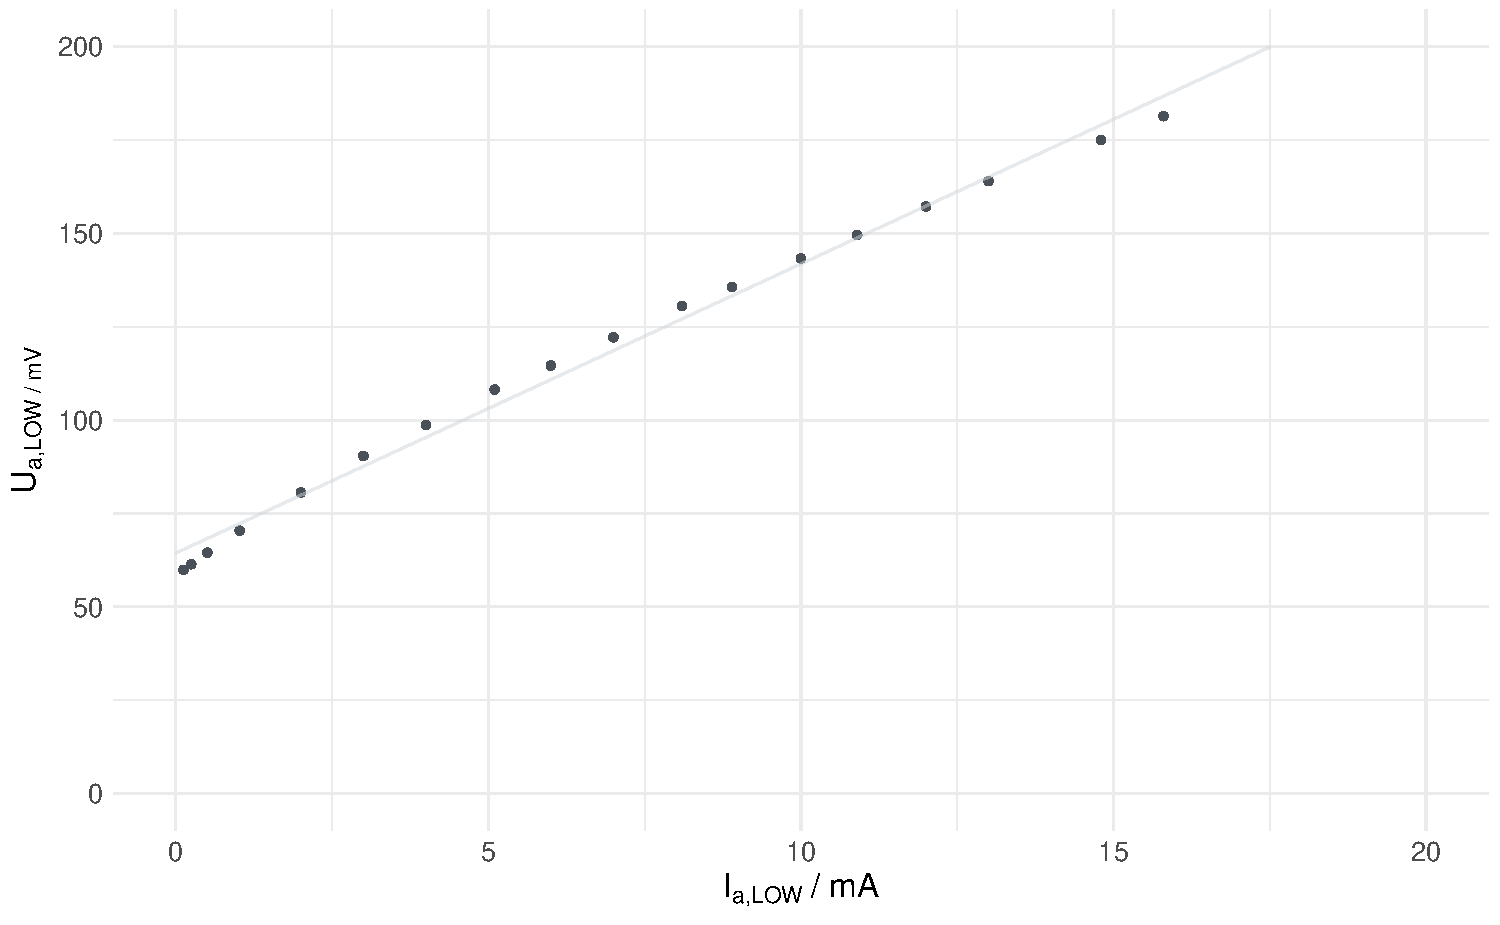
\includegraphics[width=\textwidth]{VERA/SN7400/SN7400_Ausgangskennlinie_low}
  \end{center}
  \caption{Graph der Messwerte von Ausgangs-LOW-Strom und -Spannung}
  \label{fig:graphic_low}
\end{figure}

Abbildung \ref{fig:graphic_low} zeigt den linearen Zusammenhang zwischen
Strom und Spannung bei LOW-Pegel am Ausgang, Tabelle \ref{tab:aus_low} enthält
die zugehörigen Messwerte. Mithilfe von linearer Regression
konnte eine Änderungsrate von $7.745 \, \si{\milli\volt}$ Ausgangsspannung je $1
\, \si{\milli\ampere}$ Ausgangsstrom ermittelt werden, was einem
statischen Widerstand von $7.745 \, \Omega$ entspricht.